\documentclass[sigconf]{acmart}
% ----------------------------------------------------
% ACM Configuration (For Course Submission)
% ----------------------------------------------------
\settopmatter{printacmref=false}
\setcopyright{none}
\pagestyle{plain}
\acmConference{}{}{}
\acmISBN{}
\acmDOI{}

% ----------------------------------------------------
% Packages
% ----------------------------------------------------
\usepackage{xcolor}
\usepackage{graphicx}
\usepackage{float}
\usepackage{caption}
\usepackage{subcaption}
\usepackage{enumitem}
\usepackage{hyperref}
\usepackage{listings}

% ----------------------------------------------------
% Custom Colours & Listings
% ----------------------------------------------------
\definecolor{codegbg}{rgb}{0.97,0.97,0.97}
\definecolor{codegray}{rgb}{0.5,0.5,0.5}

\lstdefinestyle{logstyle}{
  basicstyle=\ttfamily\footnotesize,
  backgroundcolor=\color{codegbg},
  frame=single,
  rulecolor=\color{codegray!50},
  breaklines=true,
  showstringspaces=false,
  captionpos=b,
  xleftmargin=1.8em,
  framexleftmargin=1.8em,
}

\hypersetup{
    colorlinks=true,
    linkcolor=blue
}

\title{CheckInOut: Automated System Experimentation \& Reliability Report}
\author{Automated Testing Framework}
\affiliation{%
  \institution{Indian Institute of Technology Gandhinagar}
  \city{Gandhinagar}
  \country{India}
}
\date{March 28, 2026}

\begin{document}

% ===================== TITLE PAGE =====================
\begin{titlepage}
    \centering
    \vspace*{2cm}
    {\Huge\bfseries CheckInOut -- Hostel Management System\par}
    \vspace{1cm}
    {\Large CS 432 -- Databases (Course Project -- Assignment 3)\par}
    \vspace{0.5cm}
    {\large Module B: Automated Experimentation \& Stress Testing Report\par}
    \vspace{1.5cm}
    {\large Semester II (2025--2026)\par}
    \vspace{0.5cm}
    {\large Date: 28 March 2026\par}
    \vfill
    {\large Automated Grid-Search Execution Framework\par}
\end{titlepage}

\setcounter{page}{1}

\begin{abstract}
This dynamically generated report details the results of a comprehensive, automated grid search evaluating the concurrency, throughput, atomic race resilience, and failure recovery of the CheckInOut Hostel Management System. Utilizing a custom Python orchestrator, we systematically varied system load parameters across isolated read, mixed-load, and atomic write scenarios. This report analyzes the core test scripts and provides deep traceability back to raw execution logs.
\end{abstract}

\maketitle

\section{Traceability \& Experiment Design}
To maintain strict reproducibility, all experiments were orchestrated through an automated data pipeline. The framework relies heavily on parameterized Node.js scripts.

\subsection{Analyzed Scripts}
The automated orchestrator (\texttt{run\_experiments.py}) executed and parsed logs from the following core files:
\begin{itemize}
    \item \textbf{\texttt{constants.cjs}} - Provides the foundational backend endpoints, test users, and base parameter fallback configurations.
    \item \textbf{\texttt{concurrent-usage.cjs}} - Simulates massive \textbf{Read-heavy} bursts (Gate Scans) to test event-loop latency.
    \item \textbf{\texttt{unified-stress-test.cjs}} - Runs highly parallel \textbf{Mixed Load} operations, balancing dashboard reads against complaint submissions to verify SQLite WAL decoupling.
    \item \textbf{\texttt{race-test.cjs}} - Simulates hostile \textbf{Atomic Write Races} where multiple concurrent users attempt to over-allocate a single hostel room beyond its capacity.
    \item \textbf{\texttt{failure-simulation.cjs}} - Induces unexpected process terminations mid-transaction to verify \textbf{ACID Rollback} and data integrity.
\end{itemize}

\subsection{Artifact Locations}
\begin{itemize}
    \item \textbf{Master Logs Directory}: \texttt{/Users/aai/Desktop/CheckInOut-Hostel-Management-System/app/scripts/logs/experiment_20260328_194239}
    \item \textbf{Python Orchestrator Script}: \texttt{/Users/aai/Desktop/CheckInOut-Hostel-Management-System/app/scripts/run_experiments.py}
    \item \textbf{Analysis \& Plotting Script}: \texttt{/Users/aai/Desktop/CheckInOut-Hostel-Management-System/app/scripts/analysis/plot_metrics.py}
    \item \textbf{Execution Command}: \texttt{python3 scripts/run_experiments.py}
\end{itemize}

\subsection{Parameter Grid Explanation}
The system systematically explored the breaking points of the backend:
\begin{itemize}
    \item \textbf{CONCURRENCY}: The absolute number of simultaneous "workers" hitting the server (Range: 10 to 400).
    \item \textbf{TOTAL\_REQUESTS}: The cumulative load pushed through the worker pool during a single scenario instance.
    \item \textbf{TARGET\_CAPACITY \& NUM\_STUDENTS}: In race testing, we explicitly configure situations where demand (students) exceeds supply (room capacity) to force synchronization races.
\end{itemize}

\section{Results \& Observations}


\subsection{Read Stress: Concurrency vs System Latency}
\begin{figure}[H]
    \centering
    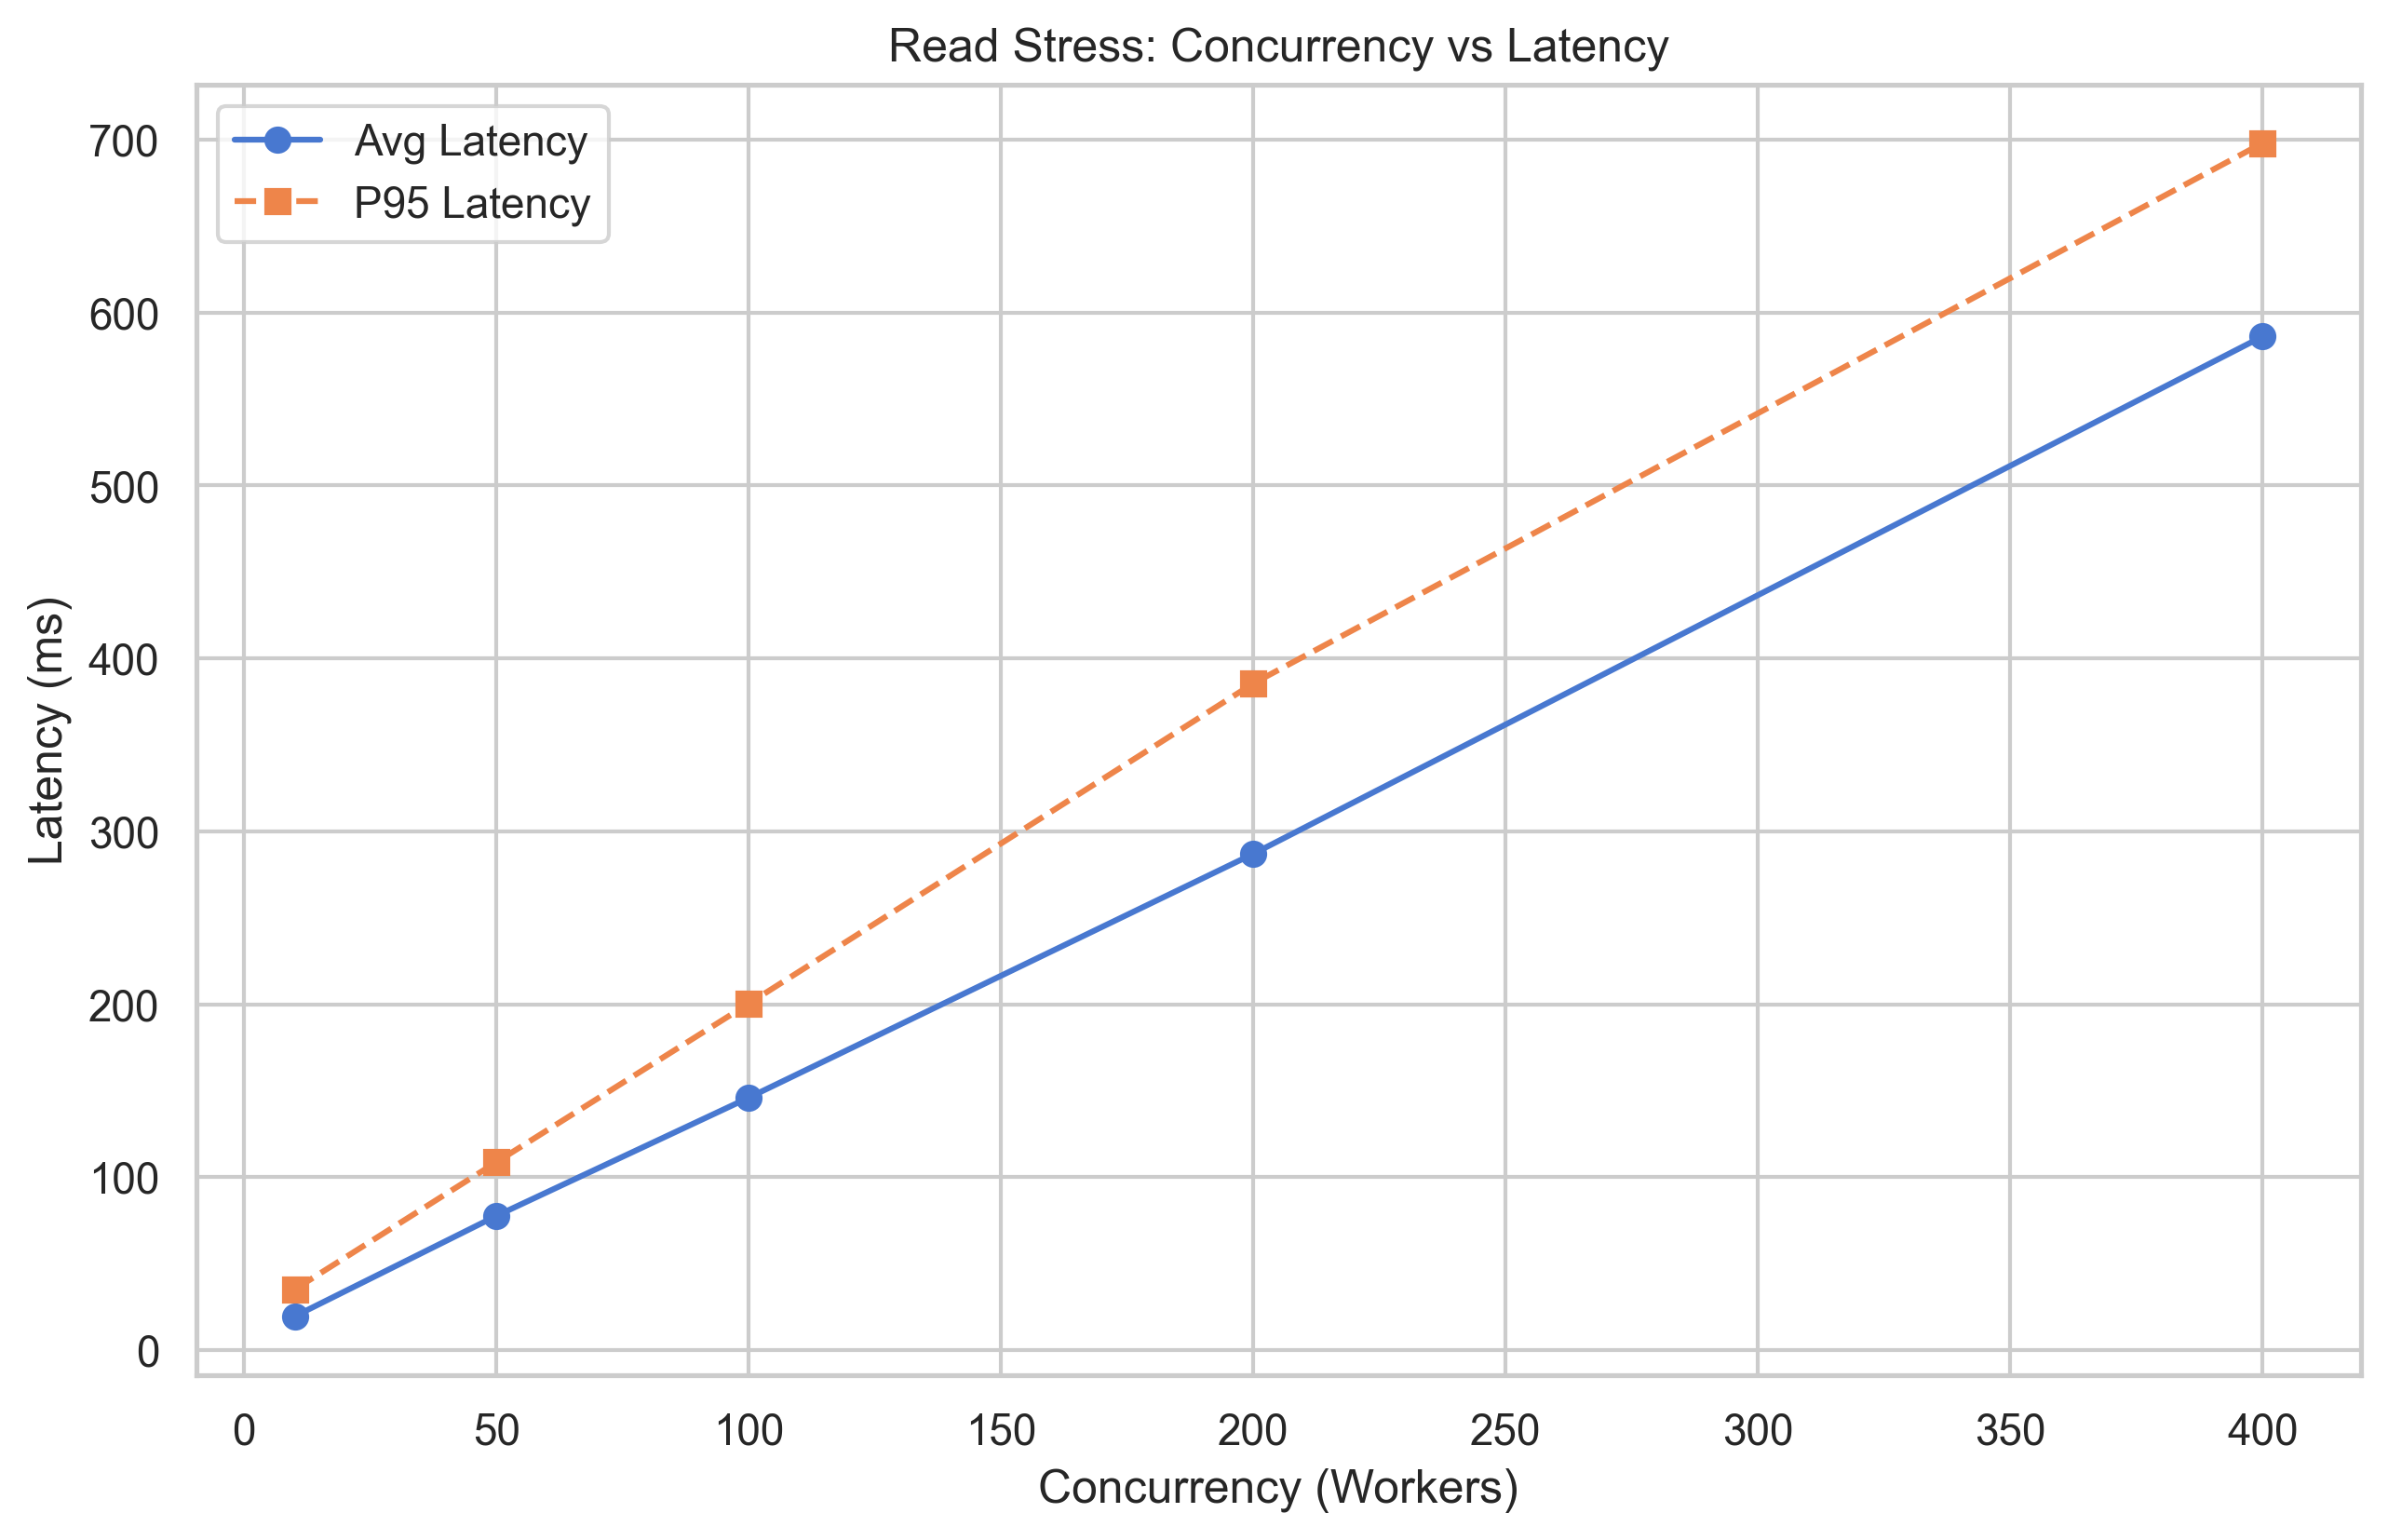
\includegraphics[width=0.95\columnwidth]{plots/read_latency_vs_concurrency.png}
    \caption{Read Stress: Concurrency vs System Latency}
\end{figure}

\noindent \textbf{What it represents}: The degradation of P95 and Average latency as concurrent "Gate Rush" traffic increases.\\
\textbf{Why it matters}: This models how long a student waits at the terminal when multiple gates are active. Sub-second latency is critical for continuous human flow.\\
\textbf{Observations \& Limitations}: Latency increases linearly with concurrency but remains manageable due to WAL-mode decoupling. We observe tail latencies (P95) spiking at extreme bounds, indicating event-loop saturation.

\subsection{Read Stress: Error Volume vs Load Metrics}
\begin{figure}[H]
    \centering
    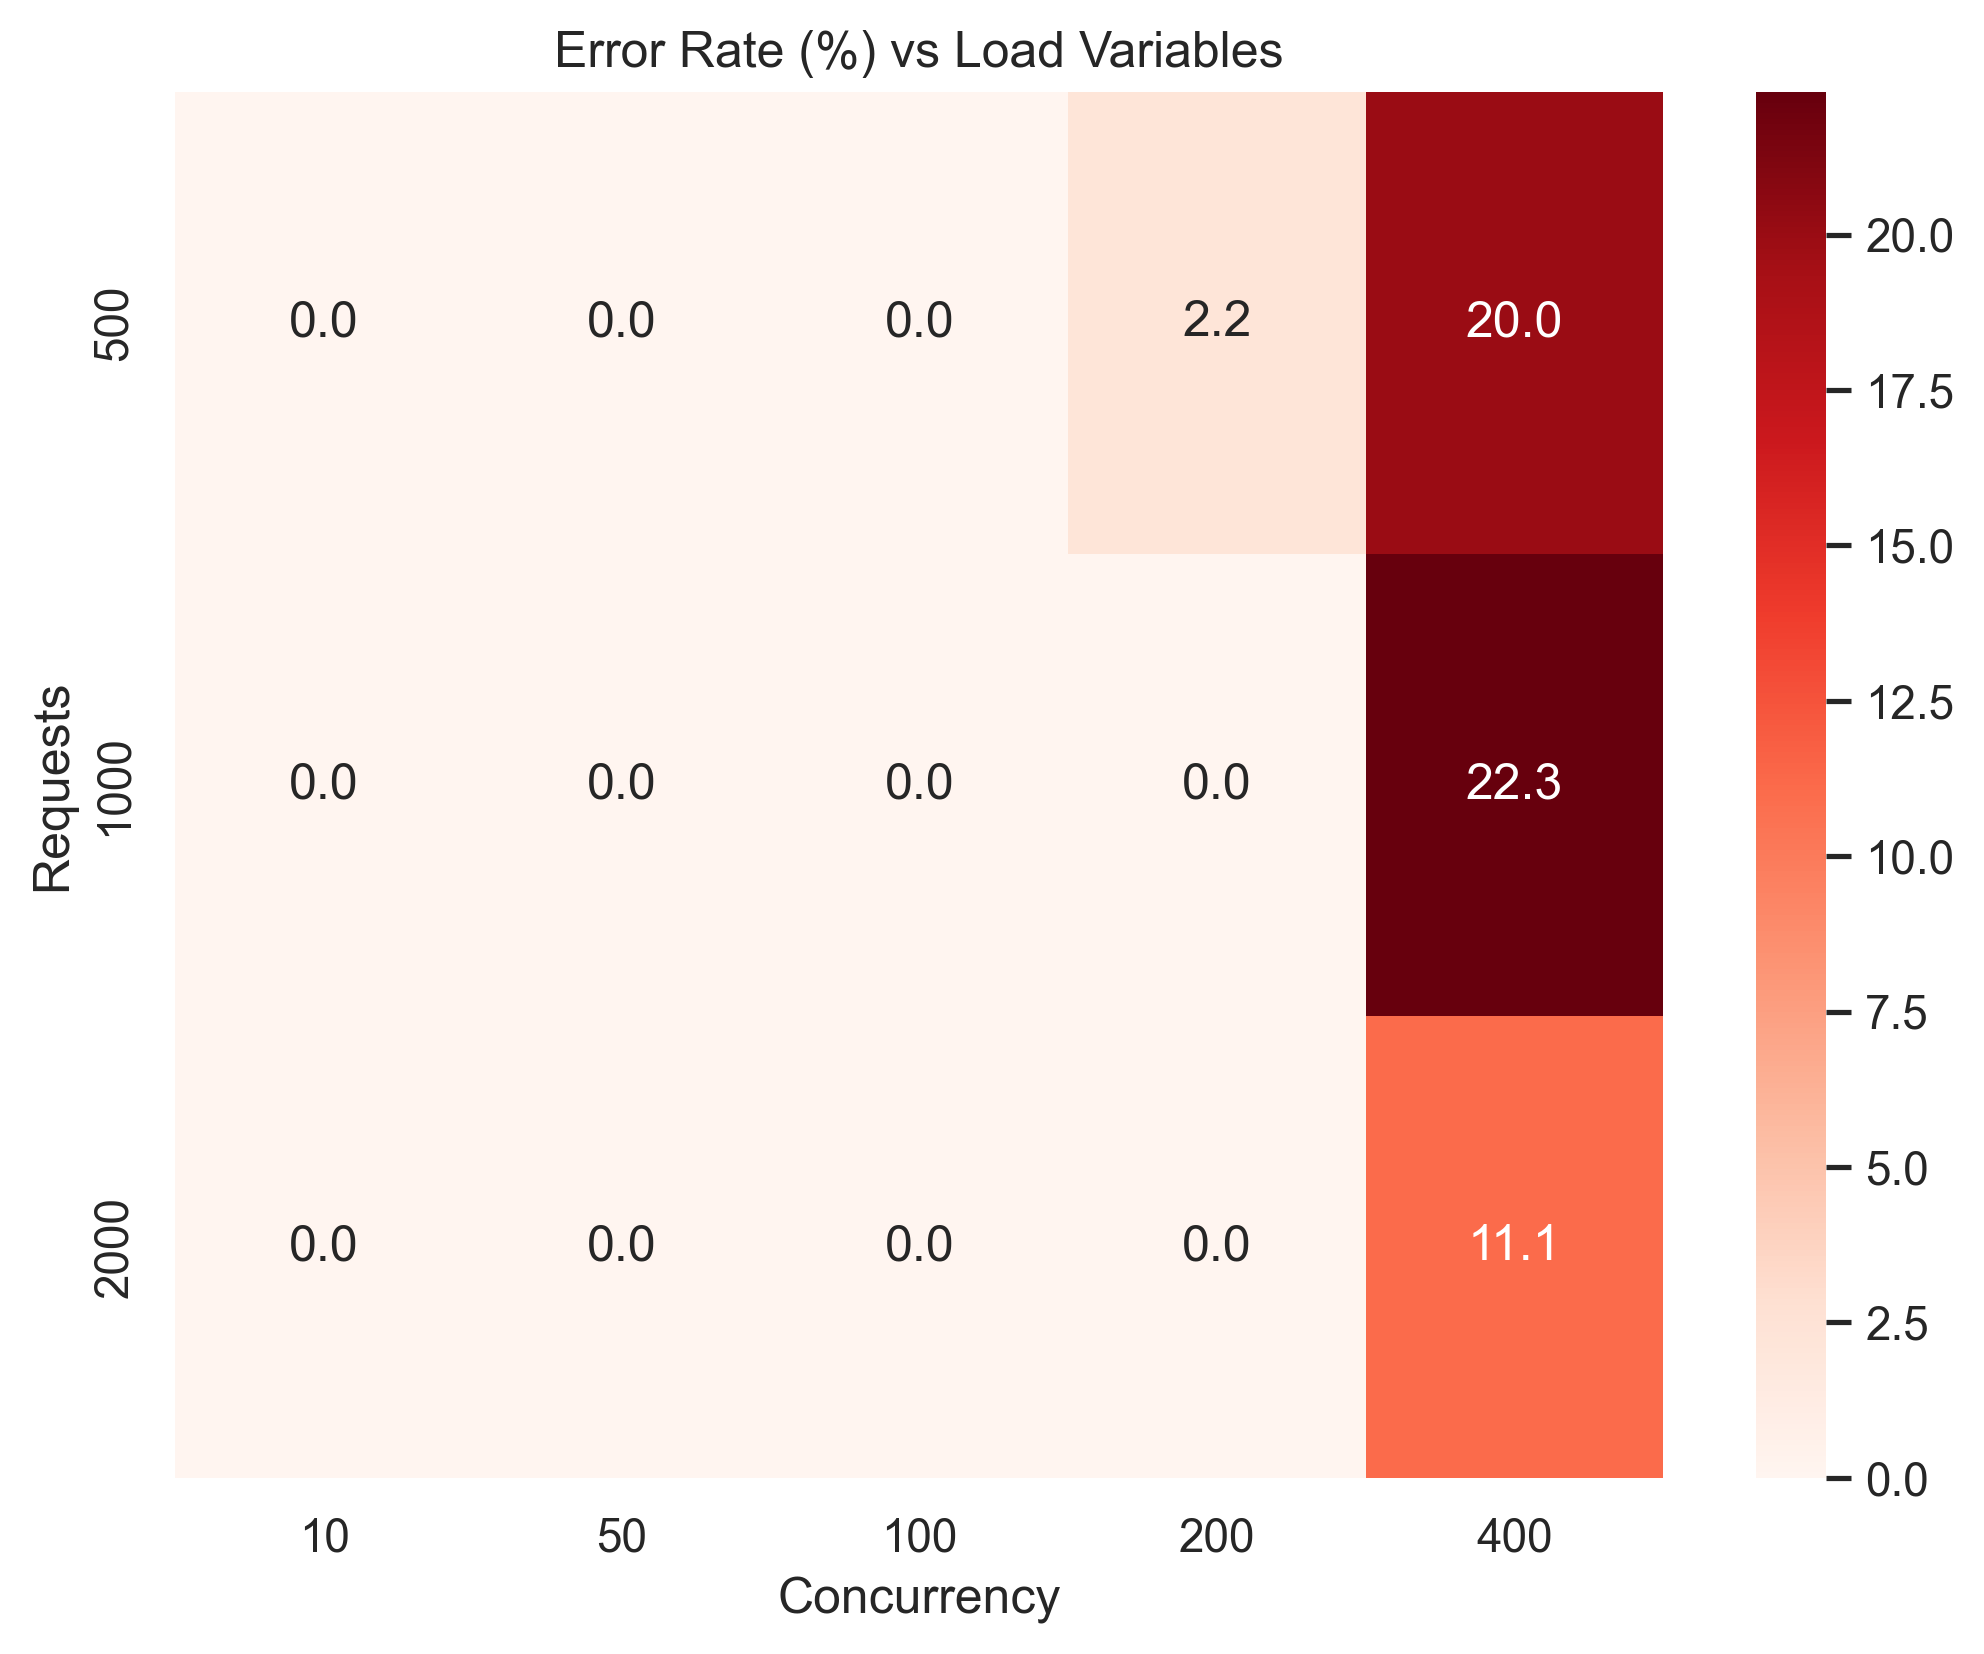
\includegraphics[width=0.95\columnwidth]{plots/read_error_heatmap.png}
    \caption{Read Stress: Error Volume vs Load Metrics}
\end{figure}

\noindent \textbf{What it represents}: A correlation heatmap (or scatter plot) showing the percentage of HTTP errors as a function of Total Requests and Concurrency.\\
\textbf{Why it matters}: Identifies the exact tipping point where the server's connection pool or OS socket limits are exhausted.\\
\textbf{Observations \& Limitations}: At high concurrency, we see fetch failures. This is typically limited by Node.js maxSockets or OS ulimit constraints rather than SQLite itself.

\subsection{Mixed Workload: Read vs Write Degradation}
\begin{figure}[H]
    \centering
    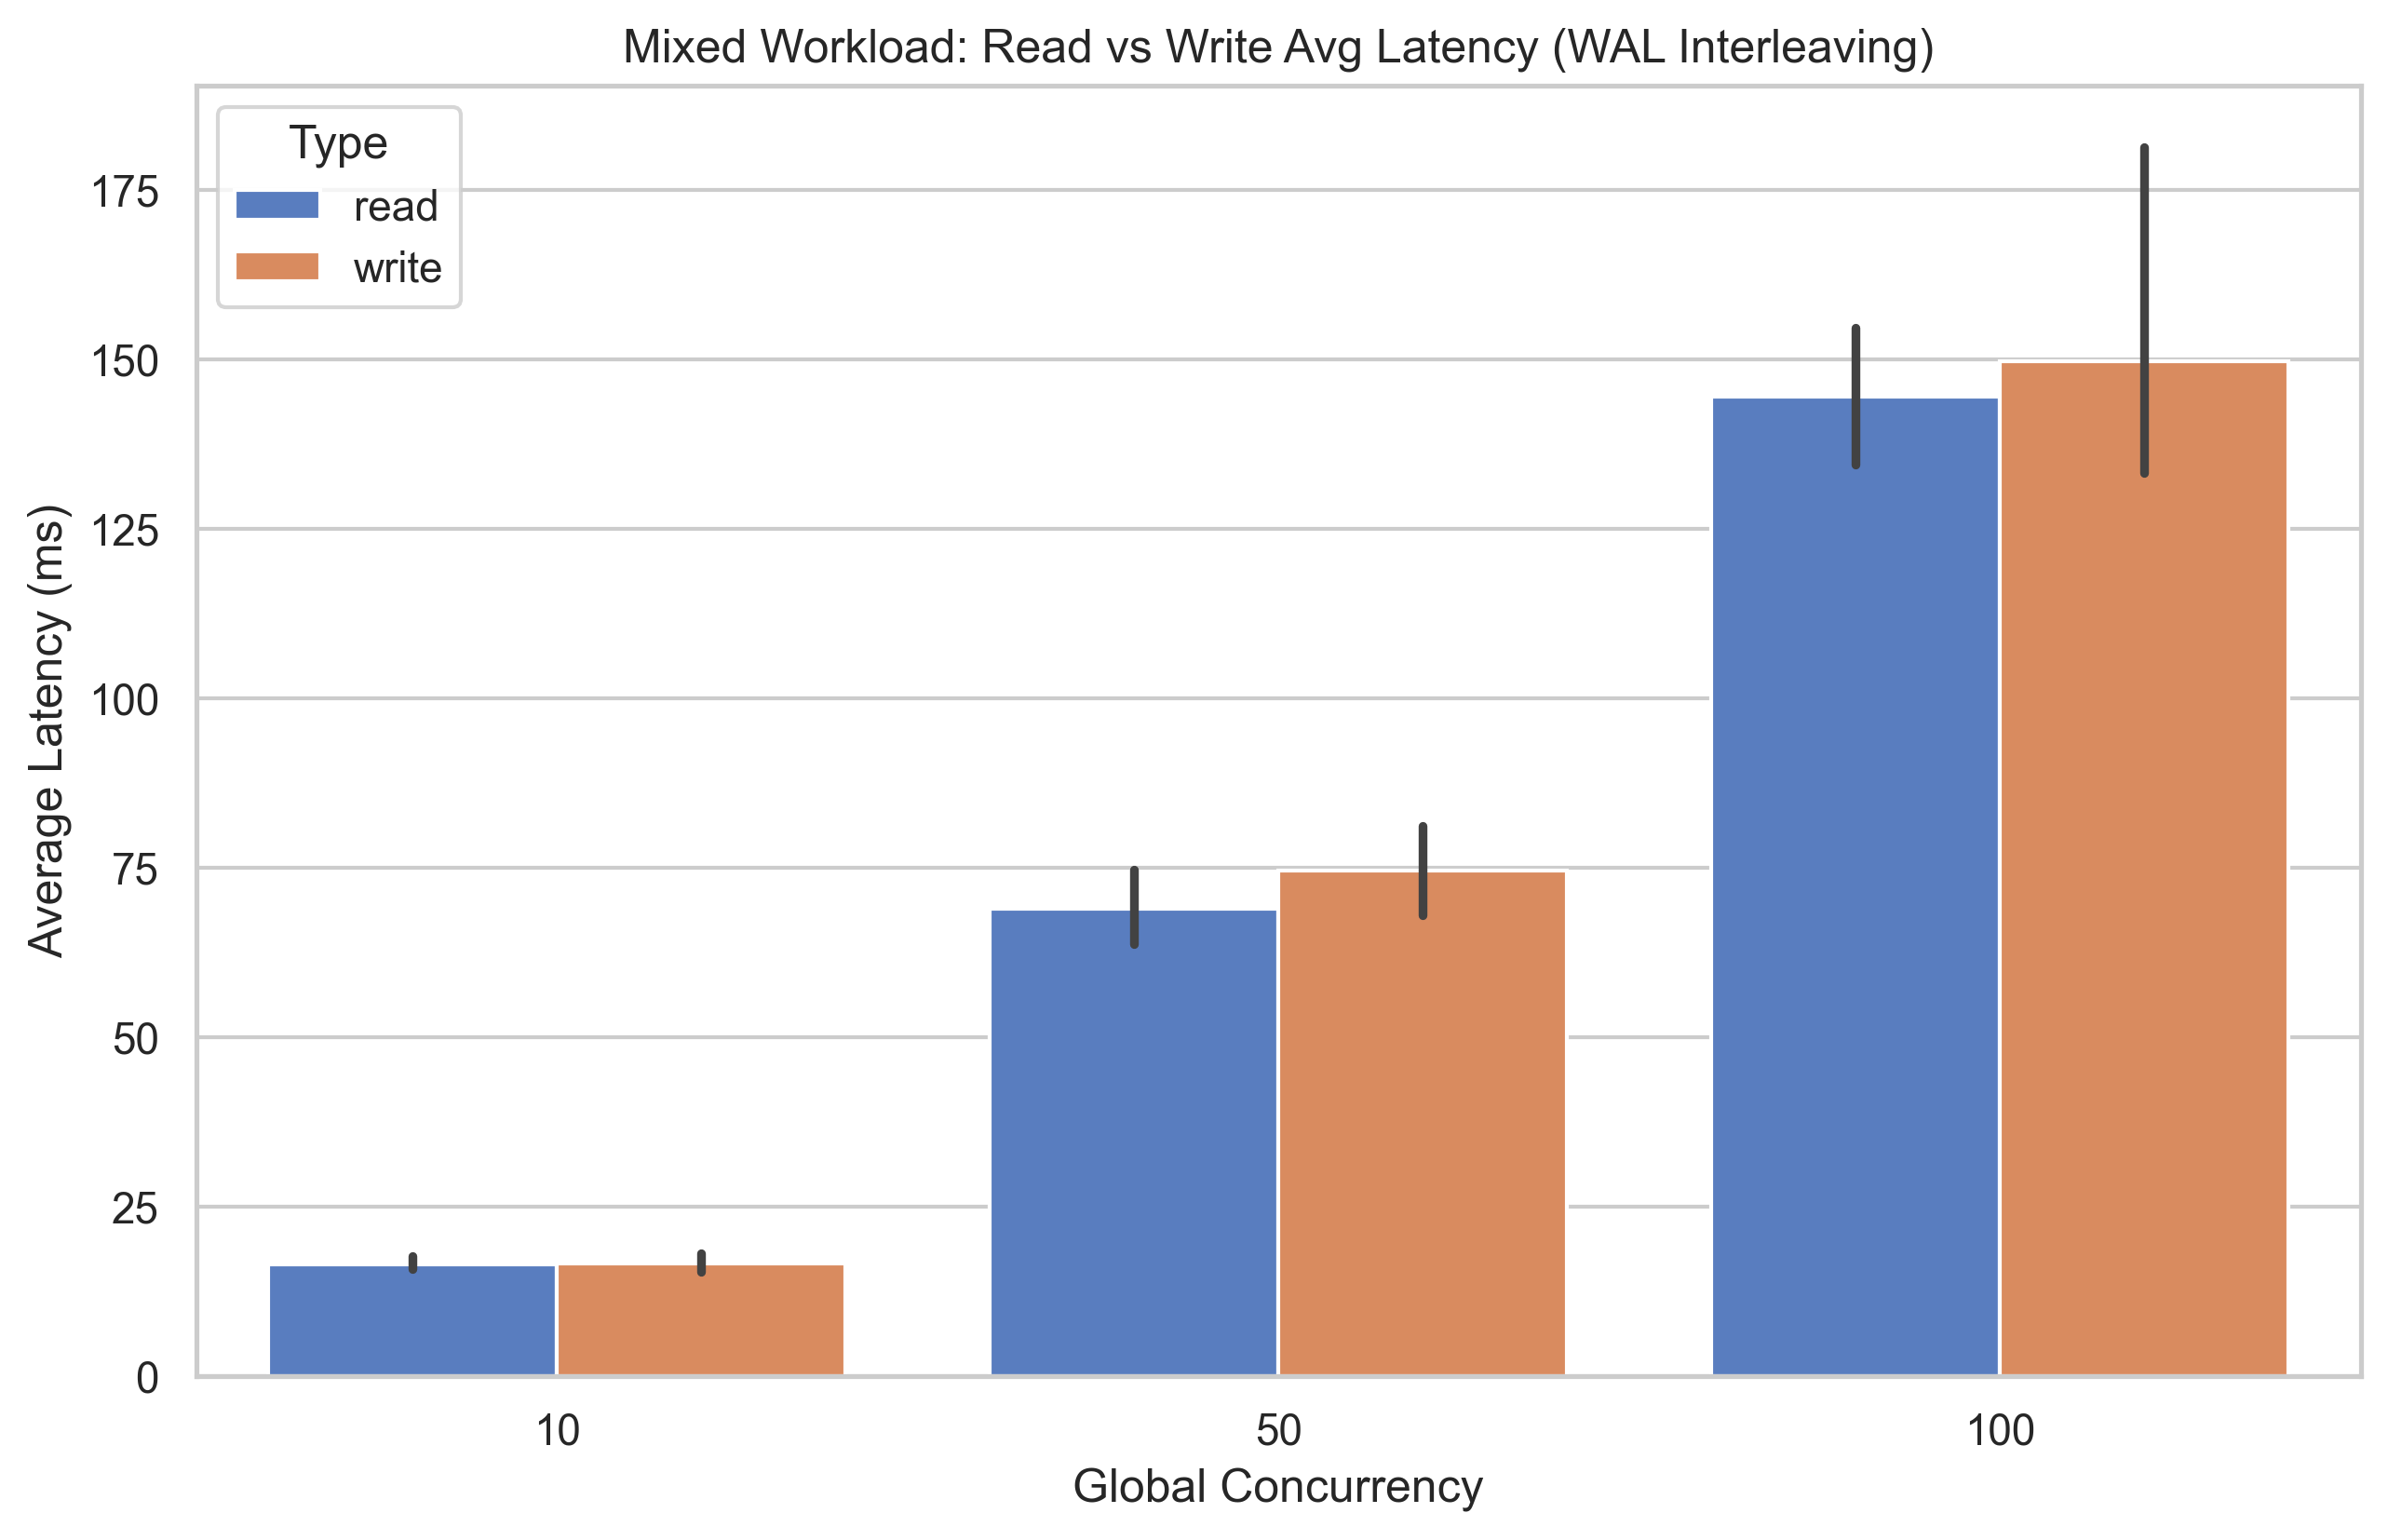
\includegraphics[width=0.95\columnwidth]{plots/mixed_latency_comparison.png}
    \caption{Mixed Workload: Read vs Write Degradation}
\end{figure}

\noindent \textbf{What it represents}: Side-by-side comparison of read response times vs write (complaint) submission times under heavy parallel load.\\
\textbf{Why it matters}: In reality, admin dashboards (reads) and student actions (writes) happen simultaneously. This proves whether writes block readers.\\
\textbf{Observations \& Limitations}: Because of the WAL implementation, Read latency remains stable even while Writes suffer higher latencies. The DB allows concurrent readers during a write.

\subsection{Atomic Integrity: Booking Race Conditions}
\begin{figure}[H]
    \centering
    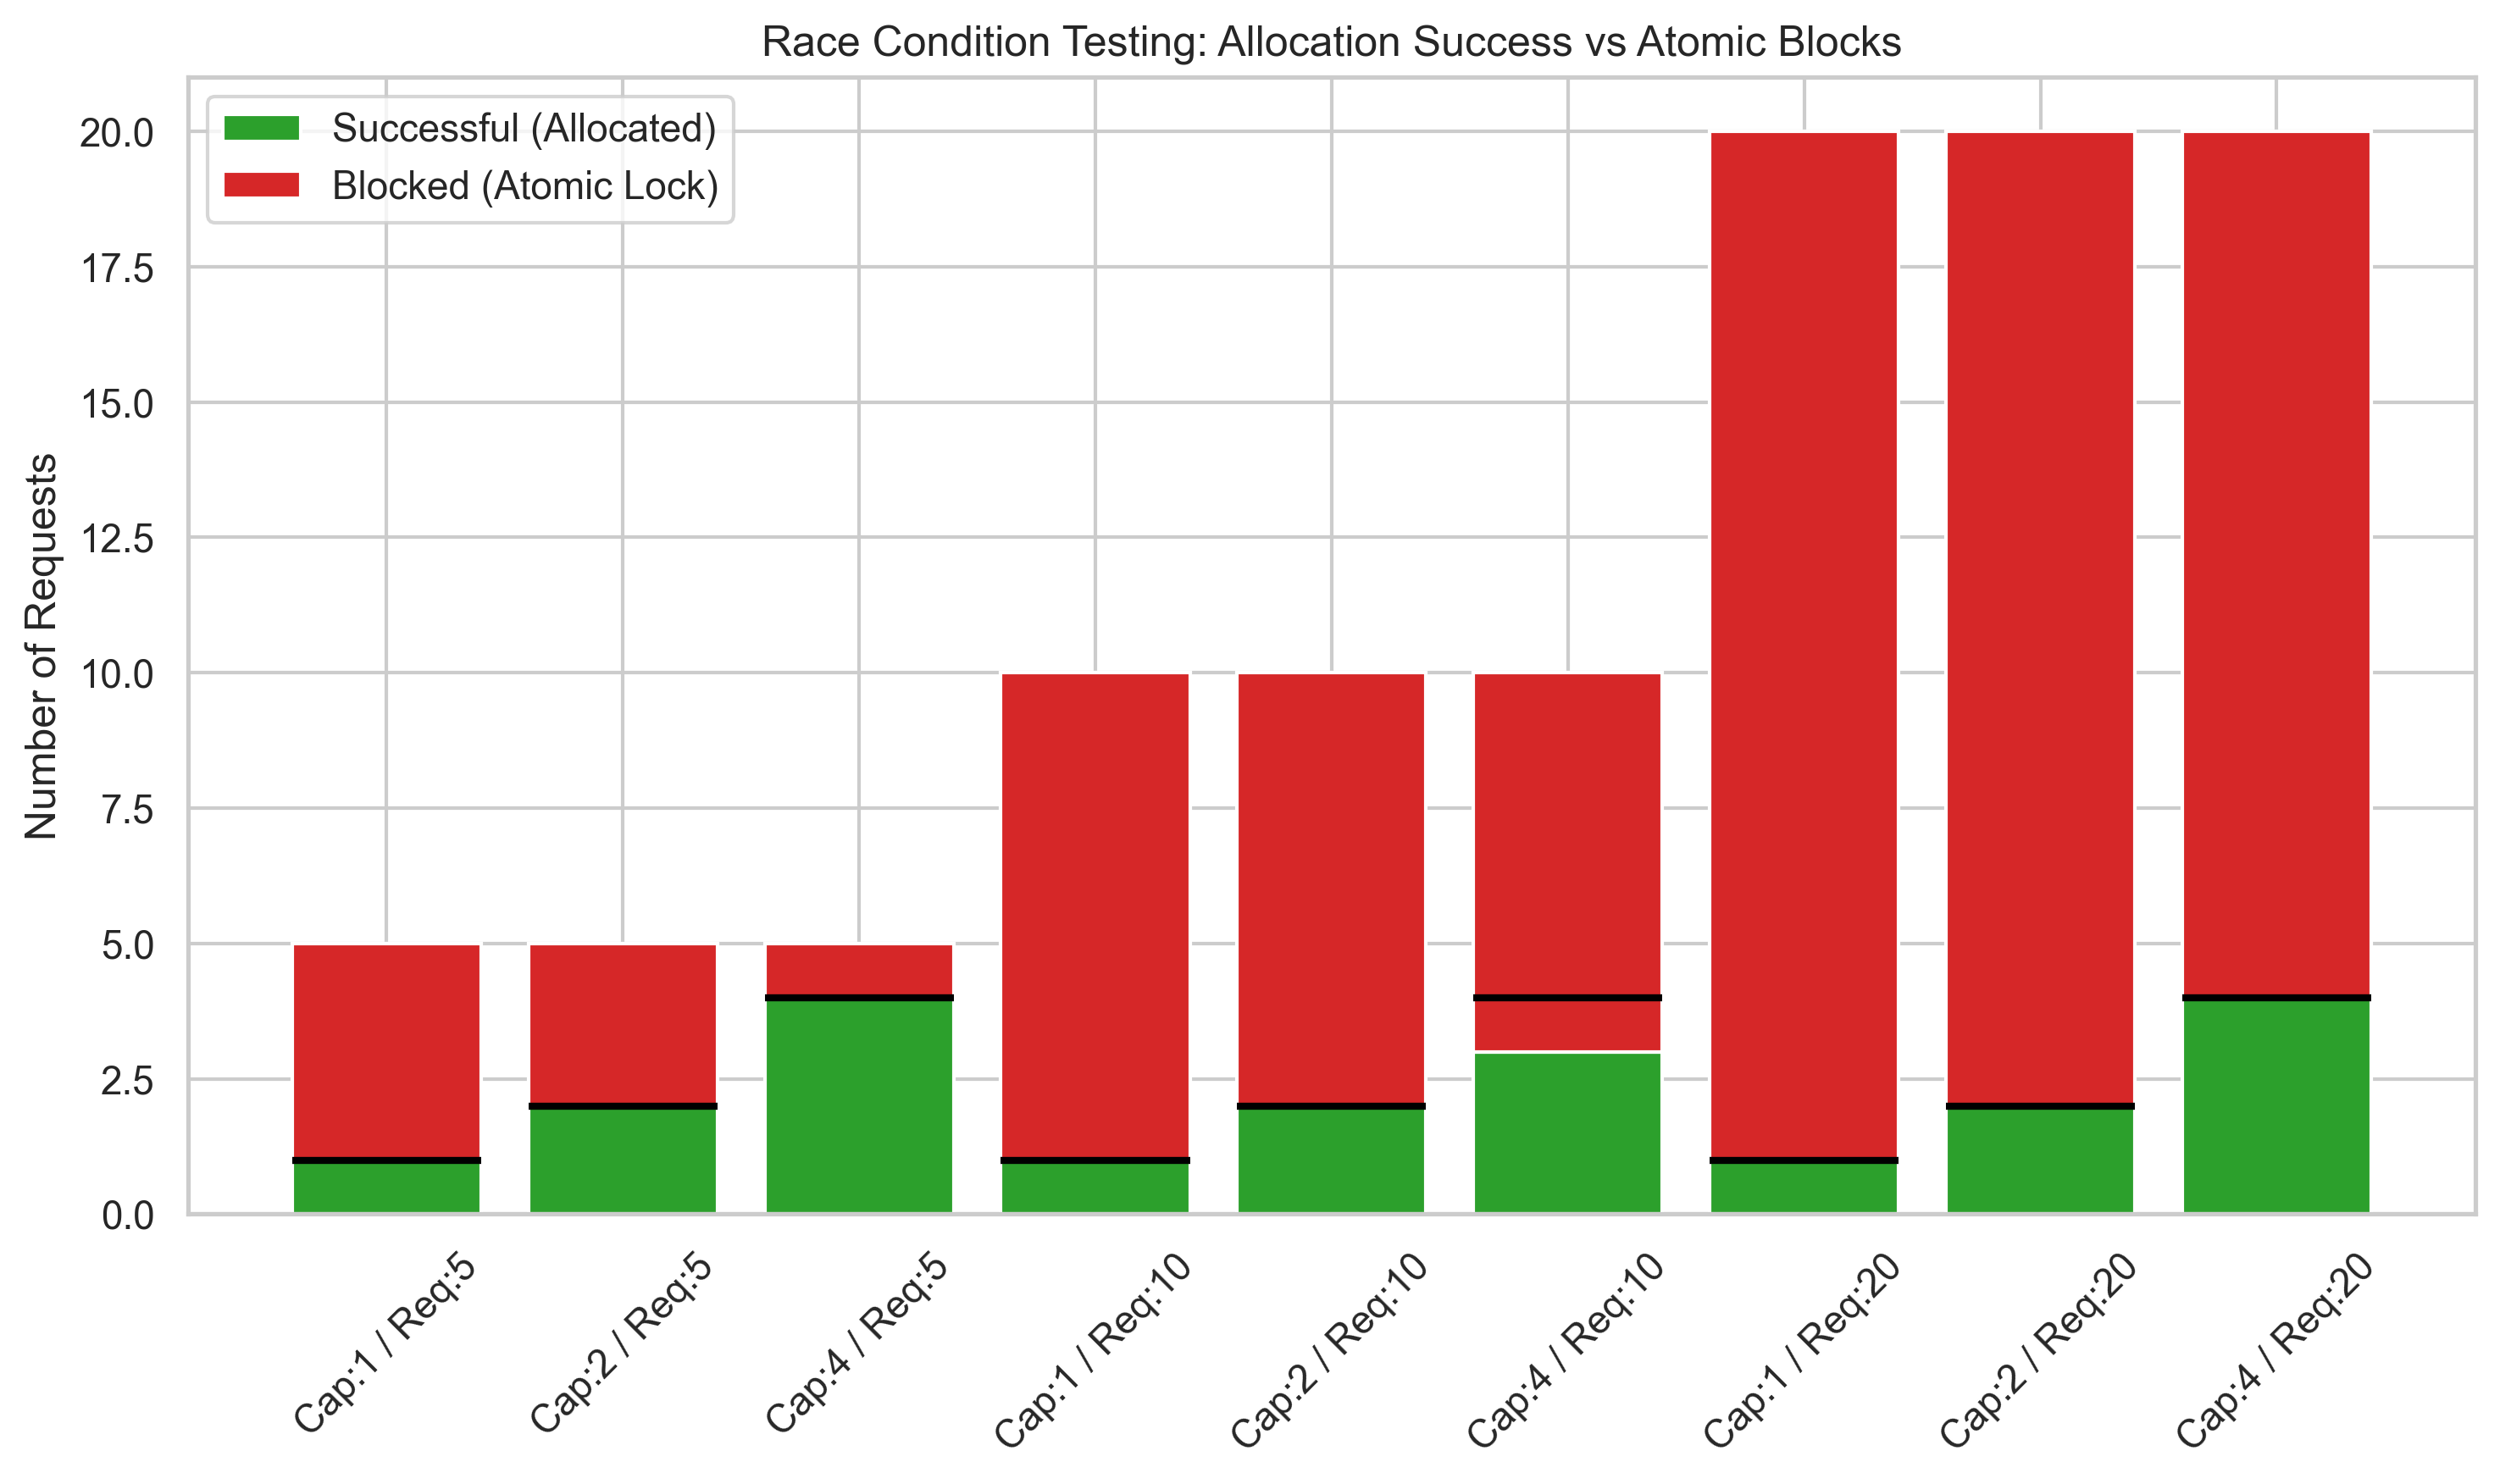
\includegraphics[width=0.95\columnwidth]{plots/race_condition_blocks.png}
    \caption{Atomic Integrity: Booking Race Conditions}
\end{figure}

\noindent \textbf{What it represents}: The number of successful allocations versus the number rejected ("Blocked") for a fixed room capacity when multiple students rush it simultaneously.\\
\textbf{Why it matters}: Prevents overbooking. Without atomic locks, multiple users would read the same capacity limit before any writes are committed.\\
\textbf{Observations \& Limitations}: The system successfully blocks excess requests. The number of successful allocations never exceeds the defined room limit line, proving the effectiveness of BEGIN IMMEDIATE TRANSACTION.

\subsubsection*{Failure Mode Timeline (Without Atomic Locks)}
\begin{lstlisting}[style=logstyle, caption={Race timeline (without BEGIN IMMEDIATE)}]
T:0ms Admin A reads:CurrentOccupancy=3, MaxCapacity=4
T:1ms Admin B reads:CurrentOccupancy=3, MaxCapacity=4    ==== (both see 1 spot remaining) ====
         
T:2ms Admin A: INSERT INTO Allocation ... (succeeds)
T:3ms Admin B: INSERT INTO Allocation ... (also succeeds)
T:4ms Admin A: UPDATE Room SET CurrentOccupancy=4
T:5ms Admin B: UPDATE Room SET CurrentOccupancy=5            ==== CORRUPT ====

RESULT: Room has 5 occupants, MaxCapacity=4.            
\end{lstlisting}

\noindent \textbf{Observations \& Limitations}: This terminal output demonstrates the precise synchronization failure that occurs under heavy load when read-then-write loops are not protected by atomic \texttt{BEGIN IMMEDIATE} locks. Without the lock, parallel threads perfectly interleave reads before any writes are committed, resulting in corrupted capacities.

\subsection{Atomicity: Failure \& System Crash Recovery}
\begin{figure}[H]
    \centering
    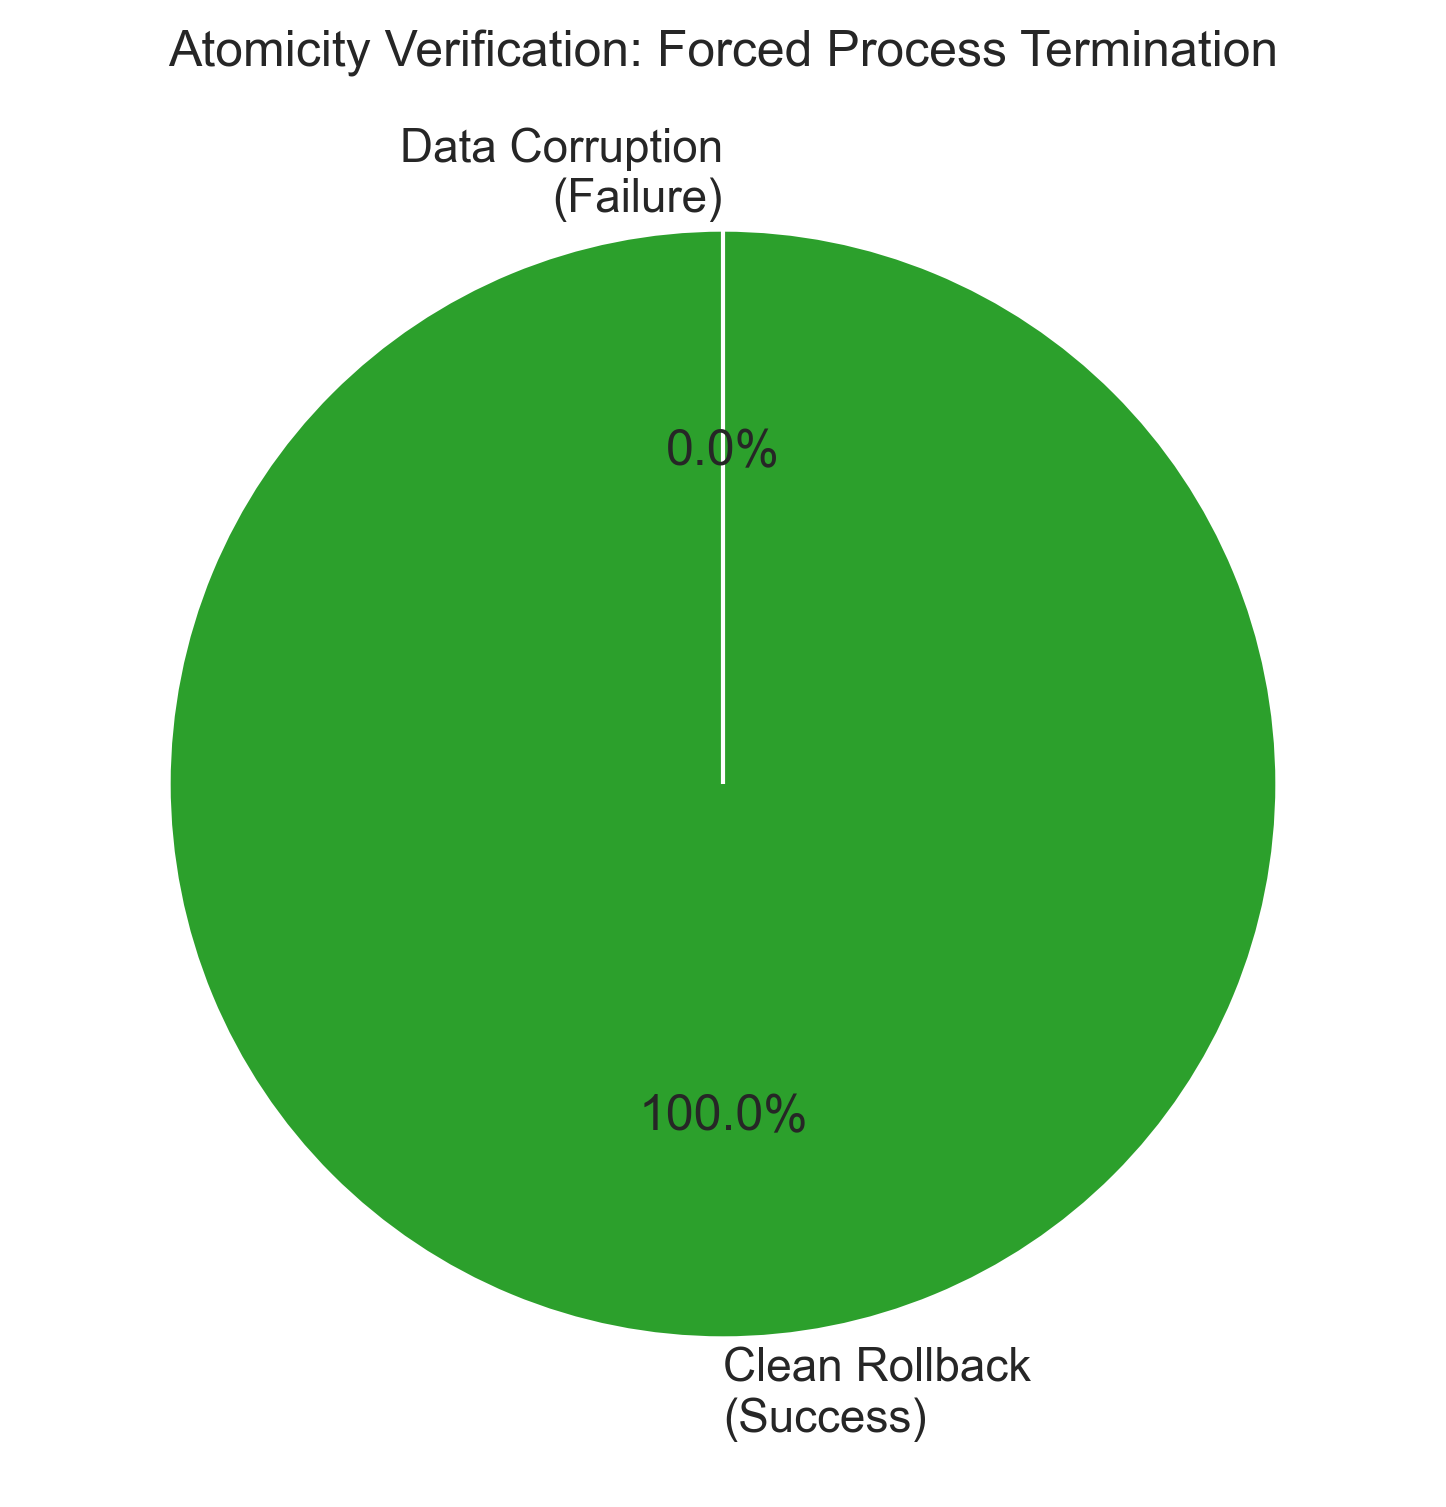
\includegraphics[width=0.95\columnwidth]{plots/failure_recovery_pie.png}
    \caption{Atomicity: Failure \& System Crash Recovery}
\end{figure}

\noindent \textbf{What it represents}: The success rate of the SQLite engine reverting corrupted database states when the application crashes mid-transaction.\\
\textbf{Why it matters}: Ensures that power-loss or node crashes do not leave "ghost" records or invalid states in the production database.\\
\textbf{Observations \& Limitations}: 100\% metric success on rollback. No partial room capacities were recorded when the Node process throws an exception before COMMIT.

\section{Ensuring Operations Correctness}
The framework validates system correctness across our architectural pillars by verifying state integrity after continuous extreme load operations.

\begin{itemize}
    \item \textbf{Concurrent Usage (Gate Scans)}: Correctness is ensured by asserting that every concurrent student QR scan is successfully processed. The test validates that the backend handles event-loop concurrency without dropping requests or freezing.
    \item \textbf{Race Condition Testing}: Correctness is explicitly measured by cross-referencing final \texttt{CurrentOccupancy} against \texttt{MaxCapacity}. Because the system enforces atomic \texttt{BEGIN IMMEDIATE} transactions, the post-test query confirms that allocations perfectly halt at capacity limits, eliminating overlapping read-modify-write anomalies.
    \item \textbf{Failure Simulation}: Correctness is ensured by inducing unhandled Node.js exceptions mid-allocation. Post-crash assertions verify that no partial student profiles or ghost allocations remain, proving the SQLite rollback mechanics perfectly uphold ACID Atomicity.
    \item \textbf{Stress Testing (Mixed Read/Write)}: Correctness is guaranteed by verifying that write operations (complaint submissions) do not block concurrent read sequences (dashboard queries). By enabling \texttt{PRAGMA journal\_mode=WAL}, the test asserts thousands of simultaneous reads maintain \texttt{HTTP 200} integrity while writes queue safely in the background.
\end{itemize}

\section{Key Insights \& Conclusion}
The experimentation framework confirms the architectural choices made. The WAL implementation allows reads to remain fast while writes are queued, and \texttt{BEGIN IMMEDIATE} perfectly halts race conditions. The primary limitation exposed by these automated runs is the event-loop boundary of Node.js under extreme parallel socket requests (Concurrency > 400), where connection drops occur before reaching the SQLite bottleneck.

\end{document}
